\chapter{Integração}
%Integração e aplicação (?)
%A aplicação do sistema é realizar o controle e monitoramento semafórico em vias urbanas, visando trazer organização e segurança ao trânsito. Estar de acordo com as normas técnicas vigentes (resoluções CET). 

Cada equipamento apresentado nesse trabalho desempenha um papel importante no controle e monitoramento da sinalização semafórica nas vias urbanas. Para que todos os processos ocorram de forma ordenada e sincronizada, é necessário que se realize a integração entre os sistemas com o controlador semafórico. 
%Essa integração pode ser dividida em duas etapas: o controle veicular e o controle de pedestres. Essas duas etapas 

\section{Controlador semafórico}

A integração dos sistemas se dá através do equipamento chamado controlador semafórico. O controlador semafórico é um sistema que tem como função a supervisão e o controle do trânsito, sendo composto por hardware e software capazes de prover uma rede semafórica inteligente e automatizada.

\begin{figure}[ht]
    \begin{center}
    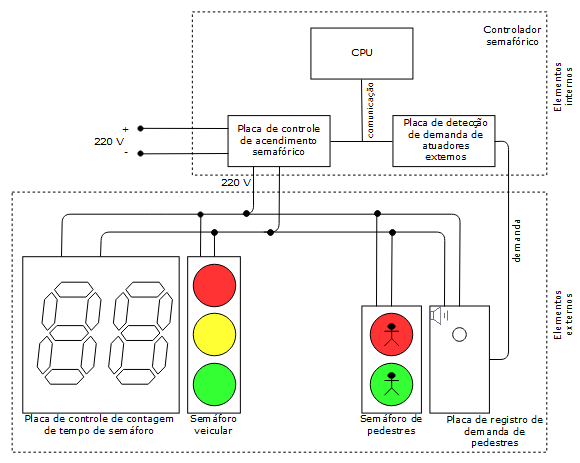
\includegraphics[width=0.7\textwidth]{figuras/diagrama_controlador.PNG}
    \end{center}
    \caption[Controlador semafórico]{Diagrama da integração do controlador semafórico.}
    \label{controlador}
\end{figure}

O controlador pode ser dividido em seus elementos internos e externos, que funcionam em conjunto para assegurar o correto funcionamento do sistema completo. A interação entre os elementos, que compoem o controlador, é mostrada na Figura \ref{controlador}. 

\subsection{Elementos internos}

Os elementos internos ao controlador são aqueles que se encontram fisicamente no gabinete do sistema. Esses elementos processam os dados medidos e recebidos dos elementos externos, e possuem comunicação com a \ac{CPU} do comtrolador.

A placa de controle de acendimento semafórico e a placa de detecção de demanda de atuadores externos são os dois elementos internos ao controlador e funcionam como interface entre a \ac{CPU} do controlador e os elementos externos, que não possuem comunicação.
A placa de controle de acendimento faz a conexão entre o controlador e os focos semafóricos (veicular e de pedestres) e a placa de contagem de tempo. A placa de detecção de demanda realiza a conexão entre o controlador e a placa de registro de demandas.

\subsection{Elementos externos}

Os elementos externos ao controlador são aqueles que não se encontram no gabinete do sistema. Esses elementos ficam à mostra e funcionam como interface entre o motorista e pedestre com o controlador semafórico. Não existem comunicação entre os elementos externos e a \ac{CPU} do controlador, portanto qualquer sinal necessário é transmitido aos elementos internos.

A placa de controle de contagem de tempo semafórico tem como finalidade indicar o tempo de acendimento restante no semáforo veicular, agindo como interface entre o usuário (motorista/pedestre) e os tempos calculados na \ac{CPU}. Já a placa de registro de demanda de pedestres possibilita a interação entre o pedestre e o controlador. Além dos dois sistemas, há ainda o foco semafórico como elemento externo ao controlador, funcionando em integração com a placa de controle de acendimento.

\section{Controle veicular}

O controle veicular é realizado pelas placa de controle de acendimento semafórico e placa de controle de contagem de tempo semafórico, assim como os focos semafóricos veiculares. A placa de acendimento é controlada pela \ac{CPU} do controlador semafórico, e é responsável pelo acendimento dos semáforos. A placa de contagem é instalada próxima ao foco semafórico. A ligação entre os elementos pode ser visto na Figura
%Mostrar esquema com ligação entre placa de acendimento, placa de contagem e foco semafórico veicular

Não há comunicação entre o foco semafórico, ou a placa de contagem, e a \ac{CPU} do controlador, pois a comunicação ocorre apenas entre a placa de acendimento e a \ac{CPU}. A única ligação entre os elementos são as linhas que levam tensão da rede elétrica da placa de acendimento até os outros dois equipamentos. A comunicação necessária se dá por essas linhas, sendo nesse caso o envio de um pulso de energia com o intuito de indicar a aproximação do fim do tempo de acendimento.

\section{Controle de pedestres}

O controle de pedestres é realizado pelas placa de detecção de demanda de atuadores externos e placa de registro de demanda de pedestres, assim como os focos semafóricos de pedestres. A placa de detecção é controlada pela \ac{CPU} do controlador semafórico, e é responsável por receber as demandas registradas pela placa de registro. A placa de de registro é instalada próxima ao ponto de travessia de pedestres. A ligação entre os elementos pode ser visto na Figura
%Mostrar esquema com ligação entre placa de detecção, placa de registro de demanda e foco semafórico de pedestres

Assim como no controle veicular, não há comunicação entre o foco semafórico de pedestres, ou a placa de registro de demandas, e a \ac{CPU} do controlador, apenas entre o controlador e a placa de detecção de demandas. As únicas ligações entre os elementos que realizam o controle de pedestres ocorrem entre o foco semafórico e a placa de registro (ligadas em paralelo na rede elétrica) e entre a placa de registro e a placa de detecção (linha de envio de demandas registradas). 